\section{Task Definition}
\label{openpsg:sec:task_definition}

We define the task, open-set panoptic scene graph generation.
Given an image $I \in \mathbb{R}^{H \times W \times 3}$, the objective of this task is to extract an open-set panoptic scene graph $G = \{O, R\}$ from the image $I$, where $H$ and $W$ are the height and width of the image.
Here:
\begin{itemize}
    \item $O = \{o_i\}_{i=1}^{N}$ represents $N$ objects segmented from the image, each defined as $o_i = \{c, m\}$, where $c$ is the object category that can belong to either predefined base object categories $C_{base}$ or undefined novel object categories $C_{novel}$.
    $m$ represents the binary mask in $\{0, 1\}^{H \times W}$ of the object.
    \item $R = \{r_{i,j} \mid i,j \in \{1, 2, \ldots, N\}, i \neq j\}$ represents the relations between objects, where $r_{i,j}$ denotes the relation between $o_i$ and $o_j$, with $o_i$ as the subject and $o_j$ as the object.
    Each relation $r$ can belong to either predefined base relation categories $K_{base}$ or undefined novel relation categories $K_{novel}$.
\end{itemize}


\begin{figure}[t]
    \centering
    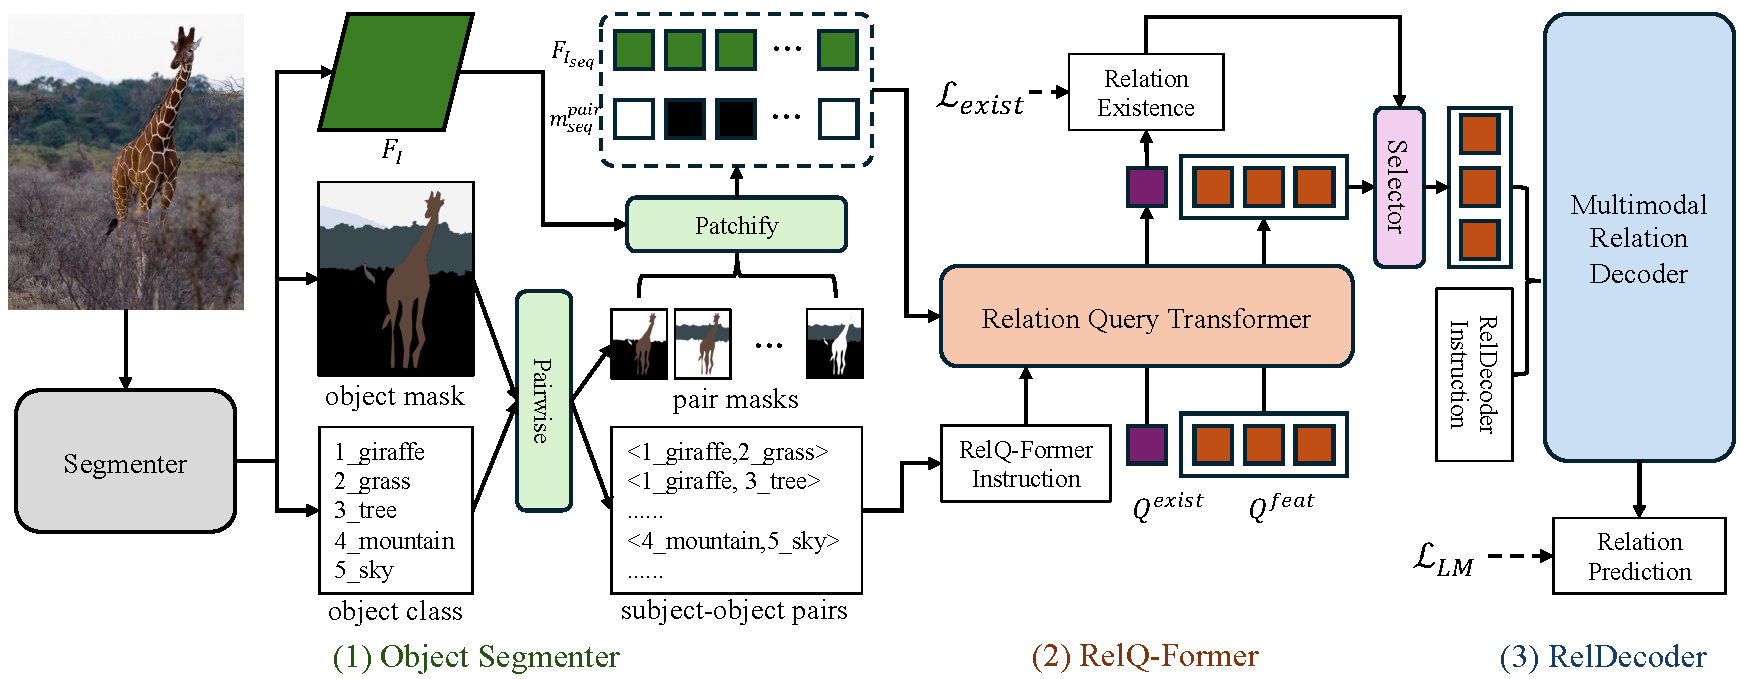
\includegraphics[width=1.0\linewidth]{Chapter5/Figures/overview.pdf}
    \caption{The overall framework of our {OpenPSG}, which comprises three components: object segmenter, relation query transformer and multimodal relation decoder.}
    \label{openpsg:fig:overview}
\end{figure}


\section{Method}
\label{openpsg:sec:method}

As illustrated in Fig.~\ref{openpsg:fig:overview}, our {OpenPSG} comprises three components: object segmenter, relation query transformer (RelQ-Former), and multimodal relation decoder (RelDecoder).
For the object segmenter (Sec.~\ref{openpsg:sec:object_segmenter}), we utilize a pretrained open-set panoptic segmentation model to transform the input image into object categories and masks, as well as visual feature representing the whole image.
Subsequently, we input the object categories, masks, and visual feature into the RelQ-Former (Sec.~\ref{openpsg:sec:rel_q_former}). Through two sets of learnable queries and complemented by designed instructions, we obtain visual features of object pairs compatible with LMMs' input format as well as judgements on potential relation existence.
Finally, only those object pairs being judged to likely have a relation are sent into the RelDecoder (Sec.~\ref{openpsg:sec:rel_decoder}) for open-set relation prediction, ultimately yielding an open-set panoptic scene graph.


\subsection{Object Segmenter}
\label{openpsg:sec:object_segmenter}
Given an image $I$, we utilize the pretrained open-set object segmenter (\eg, OpenSeeD~\cite{zhang2023simple}) to predict the objects $O$ within the image and the whole-image visual feature $F_I \in \mathbb{R}^{h \times w \times D}$. 
Here, $h$ and $w$ represent the height and width of $F_I$, and $D$ denotes the feature dimension.
The segmenter has a similar architecture to Mask2Former~\cite{cheng2022masked} includeing a pixel decoder.
The whole-image visual feature $F_I$ refers to the visual feature output by the pixel decoder.
Below, we develop the patchify module and pairwise module to process the output of the segmenter, generating the input for RelQ-Former. 

\subsubsection{Patchify Module.}
Patchify module aims to serialize visual feature $F_I$ and object masks $m$, enabling them to be processed as inputs by the RelQ-Former (Sec.~\ref{openpsg:sec:rel_q_former}).
Similar to the input patchify layer of vision transformer (ViT)~\cite{dosovitskiy2020image}, we utilize a single convolution layer to transform the extracted $F_I$ into a sequence of visual tokens $F_{Iseq} \in \mathbb{R}^{L \times D}$, where $L$ is the number of patches and $D$ is the feature dimension.
When the kernel size and stride of the convolution layer are both $p$, $L$ is calculated as $L = \frac{h}{p} \times \frac{w}{p}$.
Simultaneously, we employ nearest neighbor interpolation to each extracted object's mask $m_i$, where the size of $m_i$ is of height $\frac{h}{p}$ and width $\frac{w}{p}$, and then reshape it to a one-dimensional vector with the length $L$.
After processing all masks in the same way, we obtain the mask sequence $m_{seq} \in \{0, 1\}^{N \times L}$ for all objects.

\subsubsection{Pairwise Module.}
Pairwise module aims to construct subject-object pairs.
Given $N$ objects in the image $I$, we pairwise all objects $O$ into subject-object pairs $P = \{(o_i, o_j) | i, j \in \{1, 2, \ldots, N\}, i \neq j\}$.
The number of subject-object pairs in $P$ is $N \times (N - 1)$, which exhibits exponential growth as $N$ increases.
Consequently, we also obtain the combined subject-object pair category set $c^{pair} \in \{(c_i, c_j) | i, j \in \{1, 2, \ldots, N\}, i \neq j\}$.
We construct the mask sequences for the two objects corresponding to the indices $i$ and $j$ from $m_{seq}$ for each subject-object pair by using the logical \emph{OR} operation.
This operation is performed for all subject-object pairs, resulting in the pair mask sequence $m_{seq}^{pair} \in \{0, 1\}^{N \times (N-1) \times L}$ for the subject-object pairs, where $L$ is the number of patches.

\subsection{Relation Query Transformer}
\label{openpsg:sec:rel_q_former}
Relation query transformer, leveraging the obtained $F_{Iseq}$, $c^{pair}$, and $m_{seq}^{pair}$, employs two distinct types of queries, pair feature extraction query and relation existence estimation query, along with customized instructions.
This approach facilitates the extraction of subject-object pair features and assesses which subject-object pairs likely have relations.

\subsubsection{Pair Feature Extraction Query.}
The objective of the pair feature extraction query is to extract corresponding subject-object pair features from the whole image visual feature based on the subject-object pair masks.
A common extraction method involves mask pooling~\cite{dai2015convolutional}, which extracts features for the target subject-object pair, treating each area on the subject-object pair equally.
However, for features used in relation prediction, they should focus more on areas where interactions between objects occur. 
By leveraging attention mechanisms, we facilitate interactions among visual tokens representing different areas within the visual feature sequence $F_{Iseq}$ of a subject-object pair.
This way can enhance areas that are crucial for relation predictions.
Furthermore, inspired by \cite{liu2023improved}, we design an instruction to assist the this learnable query in understanding its purpose for extracting subject-object pair features. 

Specifically, for each subject-object pair $(o_i, o_j)$, we first input the pair feature extraction query $Q^{feat} \in \mathbb{R}^{E \times D}$ into a self-attention layer ($SA(\cdot)$), along with the pair instruction designed specifically for the pair feature extraction query.
This pair instruction is processed through a tokenizer layer to obtain $F_{Inst}^{feat} \in \mathbb{R}^{X^{feat} \times D}$, which specifies the function of the pair feature extraction query, namely ``Extracting subject-object ($c_i$, $c_j$) features from visual features according to the mask''.
Here $E$ is the token number of the pair feature extraction query, and $X^{feat}$ is the token number of the pair instruction.
Note that we also incorporate the category names of the subject and object $(c_i, c_j)$ into this pair instruction.
This operation is formulated as
% $F_{SA}^{feat} = Trunc(SA(Concat(Q^{feat}, F_{Inst}^{feat})), E)$,
\begin{equation}
    F_{SA}^{feat} = Trunc(SA(Concat(Q^{feat}, F_{Inst}^{feat})), E),
\end{equation}
where $Concat(\cdot)$ denotes the concatenation operation, $Trunc(\cdot)$ represents the truncation operation, and $E$ in this truncation operation indicates that we only extract the first $E$ features, namely the features corresponding to the pair feature extraction query.
Next, we use a mask cross-attention layer ($MaskCA(\cdot)$), with $F_{SA}^{feat}$ as the query, $F_{Iseq}$ as key and value, and $m_{seq}$ as the mask, to extract features corresponding to the subject-object pair, formulated as
% $F_{CA}^{feat} = MaskCA(F_{SA}^{feat}, F_{Iseq}, m_{seq})$.
\begin{equation}
    F_{CA}^{feat} = MaskCA(F_{SA}^{feat}, F_{Iseq}, m_{seq}).
\end{equation}
The features $F_{CA}^{feat}$ are further refined through a feed-forward network ($FFN(\cdot)$), formulated as
$F_{FFN}^{feat} = FFN(F_{CA}^{feat})$.
% \begin{equation}
%     F_{FFN}^{feat} = FFN(F_{CA}^{feat}).
% \end{equation}

By repeating this process twice, we obtain the visual features for the subject-object pair to be input into the multimodal relation decoder, $F_{I}^{pair(i,j)} \in \mathbb{R}^{E \times D}$.
We perform these operations in parallel for all subject-object pairs to obtain the corresponding features for all pairs.

\subsubsection{Relation Existence Estimation Query.}
In addition to the pair feature extraction query, we also design a relation existence estimation query to determine whether a relation likely exists between the subject $o_i$ and object $o_j$, without predicting the specific relation category.
The objective is to filter out irrelevant subject-object pairs to save the computation for subsequent LMM decoding.

Specifically, for each subject-object pair $(o_i, o_j)$, the relation existence estimation query $Q^{exist} \in \mathbb{R}^{1 \times D}$, similar to the pair feature extraction query, is input into the self-attention, mask cross-attention, and feed-forward network layers, interacting respectively with $F_{Iseq}$, $m_{seq}$ and the specially designed relation instruction.
The purpose of the relation instruction is to direct the relation existence estimation query towards determining whether a relation likely exists in the subject-object pair, \eg ``Is there a relation between $o_i$ and $o_j$?''
The relation instruction, after being processed by the tokenizer, results in $F_{Inst}^{exist} \in \mathbb{R}^{X^{exist} \times D}$, where $X^{exist}$ represents the number of tokens.
Eventually, the extracted features are input into a relation existence prediction layer, which includes a 2-layer MLP, and the predicted scores are normalized to $[0, 1]$ using the sigmoid function.
It is worth noting that we train it using binary labels indicating whether a relation exists between objects, and a selector module specified below is utilized to perform filtering during inference.

\textbf{Selector.}
The selector module implemented by 2-layer MLP is set to filter irrelvant subject-object pairs.
Only those with a score higher than the threshold $\theta$ can be input into the multimodal relation decoder.
Compared to predicting for all subject-object pairs, this can enables a 20$\times$ speedup in our experiment.


\subsection{Multimodal Relation Decoder}
\label{openpsg:sec:rel_decoder}
Multimodal relation decoder aims to utilize the subject-object pair feature $F_I^{i, j}$ extracted by the aforementioned modules, combined with an instruction guiding it to achieve open-set relation prediction.
Inspired by \cite{yue2023object, yu2023towards}, we first design a \textit{generation instruction} to perform open-set relation prediction in an autoregressive manner.
This works well, yet we find that it tends to favor common relations more or less.
Therefore, we further design a \textit{judgement instruction}, leveraging the LMMs' strong analytical and judgment capabilities.
The judgement instruction also utilizes an autoregressive manner but to judge whether a specific relation exists between objects, thereby simplifying the complexity of open-set relation prediction.
Next, we specify the two instructions, respectively.

\subsubsection{Generation Instruction.}
\label{openpsg:sec:generation_inst}
For the generation instruction, we follow the instruction design used in open-set object recognition~\cite{yu2023towards}, utilizing ``What are the relations between $c_i$ and $c_j$?''.
Here, $c_i$ and $c_j$ respectively refers to the name of the subject and object.
We convert this instruction into features $F_{inst}^{gen} \in \mathbb{R}^{X^{gen} \times D}$ using the tokenizer, where $X^{gen}$ is the token number of the generation instruction.
We input the features of this generation instruction $F_{inst}^{gen}$ together with the subject-object pair features $F_{I}^{pair(i,j)}$ into the multimodal relation decoder $Dec(\cdot)$, predicting all possible relations in an autoregressive way, formulated as 
% $r_{i,j} = Dec(Concat(F_{I}^{pair(i,j)}, F_{inst}^{gen}))$.
\begin{equation}
    r_{i,j} = Dec(Concat(F_{I}^{pair(i,j)}, F_{inst}^{gen})).
\end{equation}
If multiple relations are predicted, they are separated by the delimiter ``[SEP]''.

\subsubsection{Judgement Instruction.}
\label{openpsg:sec:judgement_inst}

Unlike generation instruction, the judgement instruction guides relation decoder to judge, based on a given relation name, whether this relation exists between the subject and object.
For example, ``Please judge between $c_i$ and $c_j$ whether there is a relation $r_k$''.
In this case, we only need the multimodal relation decoder to answer ``Yes'' or ``No'' to determine the existence of this relation.
Note that inputting the complete judgement instruction for each relation into the decoder can be costly.
Therefore, we place the relation name at the end of the instruction.
During inference we divide the judgement instruction into two parts: the section before the relation name, transformed into $F_{inst}^{judge}$ through the tokenizer, and the relation name itself, processed into $F_{inst}^{rel}$.
Benefiting from the autoregressive manner for open-set relation prediction, we initially input the subject-object pair feature $F_{I}^{pair(i,j)}$ and $F_{inst}^{judge}$ into the multimodal relation decoder, formulated as
% $F_{prefix}^{(i,j)} = Dec(Concat(F_{I}^{pair(i,j)}, F_{inst}^{judge}))$,
\begin{equation}
    F_{prefix}^{(i,j)} = Dec(Concat(F_{I}^{pair(i,j)}, F_{inst}^{judge})),
\end{equation}
which is then cached for subsequent calculations for each relation.
For each relation $r_k$, the multimodal relation decoder only needs to process $F_{prefix}$ and $F_{inst}^{rel(k)}$ to achieve relation prediction, formulated as:
% $J_{i,j,k} = Dec(Concat(F_{prefix}, F_{inst}^{rel}))$,
\begin{equation}
    J_{i,j,k} = Dec(Concat(F_{prefix}^{(i,j)}, F_{inst}^{rel(k)})),
\end{equation}
where $J_{i,j,k}$ represents the judgement for $(o_i, r_k, o_j)$ triplet.
When $J_{i,j,k}$ is ``Yes'', it indicates that the relation $r_k$ exists between $o_i$ and $o_j$; otherwise, it does not exist.
Through this approach, we can maintain the same prediction time as with the generation instruction.

We perform the aforementioned process for all subject-object pairs that may have a relation, ultimately achieving open-set relation prediction.
For method using generation instruction, we denote it as OpenPSG-G, and for those using judgement instruction, as OpenPSG-J.
In next section, OpenPSG by default refers to the latter.

\subsection{Loss Function}
\label{openpsg:sec:loss_function}
During the model training, there are two losses involved:
the binary cross-entropy loss $\mathcal{L}_{exist}$ for estimating the existence of a relation using the relation existence estimation query in the relation query transformer, and the cross-entropy loss $\mathcal{L}_{LM}$ consistent with language model training used by the multimodal relation decoder.
The total loss is:
$\mathcal{L} = \lambda \mathcal{L}_{exist} + \mathcal{L}_{LM}$,
% \begin{equation}
%     \mathcal{L} = \lambda \mathcal{L}_{exist} + \mathcal{L}_{LM},
% \end{equation}
where $\lambda$ is a weight factor.
